\documentclass{article}
\usepackage[UTF8]{ctex}
\usepackage{tikz}
\usepackage{amsmath}
\usepackage{hyperref}
\usepackage{titlesec}
\usepackage[total={7in,10in}]{geometry}
\usepackage{amssymb}
\usepackage{siunitx}
\usepackage{mathrsfs}
\usepackage[version=4]{mhchem}
\usepackage{caption}
\usepackage{subcaption}
\usepackage[RPvoltages]{circuitikz}

\newcounter{para}
\newcommand\mypara{\par\refstepcounter{para}(\thepara)\space}
\titleformat{\section}[block]{\Large\bfseries\filcenter}{}{0em}{}
\renewcommand\thesection{}
\renewcommand\thesubsection{\protect\setcounter{equation}{0}\protect\setcounter{para}{0}第 \arabic{subsection} 题}

\title{hs\_phys\_probs 003}
\author{詹有丘}
\date{}

\begin{document}

\maketitle

\subsection{原电池}
氧化还原反应是物质得或失电子的反应. 它可以用于制造化学电池.

\mypara
考虑还原 (正向) / 氧化 (逆向) 反应 $\ce{A + e- <=> B}$.
在某种条件 (浓度, 压强, 温度等) 下, 反应正向进行 $\SI{1}{mol}$
产生的 Gibbs 能变化量为 $\Delta G_\mathrm m$.
现在考虑某个装置, 使物质 A 和物质 B 相接触,
并将这个装置接入某个可以帮助电荷在 A-B 体系外部被搬运的回路中.
当反应发生时, A-B 体系减少的内能被完全转化为电能
(即 A-B 体系与外界的能量交换完全以电功的形式完成, 没有机械功和热传递),
环境条件 (压强, 温度) 不变, 且这是个可逆过程.
若以 A 端为负极, 以 B 端为正极,
求当反应发生时其产生的电动势 $E_{\mathrm A/\mathrm B}$.

\mypara
我们利用这一点制造铜锌原电池.
铜锌原电池由 $\ce{CuSO4}$ 溶液, $\ce{ZnSO4}$ 溶液以及分别插在其中的
$\ce{Cu}$ 固体和 $\ce{Zn}$ 固体组成.
在两个溶液之间有盐桥连接, 使它们能交换 $\ce{SO4^{2-}}$.
负载的两端分别接在 $\ce{Cu}$ 固体上和 $\ce{Zn}$ 上.
盐桥内有电阻 $r=\SI{1.00}{\ohm}$.
在某种条件下, 我们有下面的热化学数据:
\begin{gather*}
	\ce{\frac12Cu^{2+}(aq) + e- <=> \frac12Cu(s)},\qquad
	\Delta G_\mathrm m=-\SI{4.78}{eV}\cdot N_\mathrm A;\\
	\ce{\frac12Zn^{2+}(aq) + e- <=> \frac12Zn(s)},\qquad
	\Delta G_\mathrm m=-\SI{3.68}{eV}\cdot N_\mathrm A.
\end{gather*}
将电池接上纯电阻负载 $R=\SI{5.00}{\ohm}$,
分别求阳极 (氧化反应) 与阴极 (还原反应) 的功率 (注意正负号), 精确到三位有效数字.

\mypara
考虑一个三电极原电池.
三个电极分别为 $\ce{Zn^{2+}}$-$\ce{Zn}$ 体系,
$\ce{Cu^{2+}}$-$\ce{Cu}$ 体系,
$\ce{Ag^+}$-$\ce{Ag}$ 体系.
三个溶液两两之间以具有电阻 $r=\SI{1.00}{\ohm}$ 的盐桥连接.
在某种条件下, 上一问中的热化学数据仍然成立, 另外,
\begin{equation*}
	\ce{Ag+(aq) + e- <=> Ag(s)},\qquad
	\Delta G_\mathrm m=-\SI{5.24}{eV}\cdot N_\mathrm A.
\end{equation*}
为该原电池接入负载 $R_{\ce{Zn}\text-\ce{Cu}}=\SI{5.00}{\ohm}$,
$R_{\ce{Cu}\text-\ce{Ag}}=\SI{6.00}{\ohm}$,
$R_{\ce{Ag}\text-\ce{Zn}}=\SI{7.00}{\ohm}$.
求 $\ce{Cu^{2+}}$-$\ce{Cu}$ 体系的功率, 精确到三位有效数字.
判断它正在发生氧化反应还是还原反应.

\subsection{步步高升}

Kat 踩着高跷在与水平面的夹角为 $\alpha\in\left(-\frac\pi2,\frac\pi2\right)$ 的斜坡上走路,
$\alpha>0$ 表示上坡, $\alpha<0$ 表示下坡.
高跷始终在与斜坡垂直的平面内运动.
将 Kat 视为质量为 $m$ 的质点, 将高跷视为轻硬细杆. 称杆的末端为``脚''.
每次开始迈步时, 斜坡给予后脚大小为 $\eta m\sqrt{gl}$ 的瞬时冲量, 使这一结构从静止开始运动;
每次结束迈步时, 斜坡给予前脚一个瞬时冲量, 使这一结构静止.
每次迈步的过程中, 一只脚不与地面接触, 另一只脚始终与地面接触且不滑动
(即地面与脚之间的静摩擦系数 $\mu$ 足够大).
当脚与地面接触时, 其到 Kat 的距离保持为 $l$.
Kat 的步幅 (当两只脚同时与斜坡接触时它们之间的距离) 恒定为 $2\xi l$,
其中 $\xi\in\left(0,1\right)$.

\mypara
求 $\mu$ 的范围.

\mypara
在 $\xi$-$\alpha$ 平面中,
求能让 Kat 按题目所说的方式走路的区域的面积.

\mypara
Kat 会在每次前脚落下的同时迈出后脚.
求 Kat 的平均速度的大小与 $\sqrt{gl}$ 的比值, 用 $\alpha,\xi,\eta$ 表示.
可以保留积分号.

\subsection{帮助 Kat}

本题中可以自行按需引入一些常数.

\mypara
考虑等温大气模型: 温度不随海拔改变.
求大气密度 $\rho$ 随海拔 $z$ 的函数关系.

\mypara
Kat 想要研究在力场 $F\!\left(z\right)$ 的作用下物体由静止开始竖直下落的运动,
它在下落的过程中还会受到正比于大气密度 $\rho$ 和运动速度的平方 $\dot z^2$ 的阻力.
帮 Kat 写出这一运动的微分方程.

\mypara
Kat 看到你写下的方程后皱了皱眉: 它是一个二阶的微分方程.
但你自信地拍了拍胸脯, 说只需要令 $v:=\dot z$, 就可以将原本的二阶微分方程化为一阶微分方程.
帮 Kat 写出这个一阶的微分方程.

\mypara
Kat 看到你写下的新的方程后皱了皱眉: 它是一个非线性的微分方程.
但你自信地拍了拍胸脯, 说你可以找到一个 $\varphi\!\left(z\right)$,
使得令 $u:=\varphi\!\left(z\right)v$ 后就可以将原本的非线性微分方程化为线性的.
帮 Kat 写出这个线性的微分方程.

\mypara
Kat 觉得你很厉害, 于是你决定帮人帮到底.
帮 Kat 写出 $z\!\left(t\right)$ 的形式, 从而将求解微分方程的问题约化为积分问题.

\subsection{宏观 van der Waals 力}

1937 年, London 指出, van der Waals 力是分子间的七次方反比力.
同年, Hamaker 通过积分给出了两个匀质的宏观球之间的 van der Waals 力.
现在我们来复现一下 Hamaker 当年的成果.

\mypara
有两个匀质球, 半径分别为 $r_1$ 和 $r_2$, 球心之间距离为 $z$, 分子数密度分别为 $q_1$ 和 $q_2$.
分别来自两个球的分子之间的吸引力反比于两个分子之间的距离的七次方, 比例系数为 $6\lambda$.
求这两个球之间的吸引力的大小.
(至少将其化简至你能自信地指着它说 ``我一定能用手把它积出来'' 的程度.)

\mypara
有一块具有厚度为 $t$ 的无限大匀质平板, 以及一个半径为 $R$ 的匀质球.
这两个物体之间的间隙为 $d$.
这两个物体中的分子数密度都为 $q$, 分子间作用力仍然是比例系数为 $6\lambda$ 的七次方反比力.
求这两个物体之间的吸引力的大小.
(描述算法即可, 至少到能自信地说 ``我一定能用手把它算出来'' 的程度.)

\subsection{Moiré 纹}

考虑这样一种``光栅'', 它们像寻常的衍射光栅一样有密集分布的条纹, 用于遮挡光线.
我们所使用的光的波长的尺度远小于条纹的细节, 所以实际上无法观察到衍射现象.
当一束均匀的平行光垂直射入光栅时, 光栅背后的光屏上会展示出条纹.
它们不是光的干涉或衍射条纹, 暗纹的出现仅仅是因为本应到达该处的光被光栅上的条纹遮挡.
当我们远远地观看光屏时, 因为眼睛的辨别能力有限 (即条纹间距远小于 Rayleigh 判据的要求),
实际上观察到的是一片亮度随空间分布的光斑, 越暗的地方条纹越密.
我们定义观察到的光斑在 $\left(x,y\right)$ 处的亮度为,
在 $\left(x,y\right)$ 处取的一块小面积 $\mathrm dS$ (虽然很小, 但其尺度远大于条纹的细节)
上未被条纹遮挡的部分的面积占比.

\mypara
现在我们制作了两个相同的光栅,
光栅上均匀分布着平直的条纹, 条纹宽度都为 $d$, 条纹之间的间隙都为 $p$.
现在将两个光栅倾斜摆放, 使得它们的条纹与 $x$ 轴的夹角分别为 $\theta$ 和 $-\theta$.
两个光栅关于 $y$ 轴对称.
将这两个倾斜摆放的光栅贴在一起后得到一个新的光栅.
求均匀的平行光垂直通过这一光栅之后光屏上得到的亮度分布 $I\!\left(x,y\right)$.
量级 $d\sim p\ll\sqrt{\mathrm dS}\ll d/\theta$.

\mypara
现在我们制作了两个相似的光栅, 光栅上分布着同心圆形状的条纹.
其中一个光栅的条纹的宽度和条纹之间的间隙都为 $d_+$, 条纹的圆心在 $\left(a,0\right)$.
另一个光栅的条纹的宽度和条纹之间的间隙都为 $d_-$, 条纹的圆心在 $\left(-a,0\right)$.
将这两个光栅贴在一起后得到一个新的光栅.
求均匀的平行光垂直通过这一光栅之后在光屏上得到的亮度分布 $I\!\left(x,y\right)$.
量级 $d\sim\left|a\right|\ll\sqrt{\mathrm dS}\ll\sqrt{x^2+y^2}$.

\mypara
接上一问, 在极坐标下求暗纹中心的曲线方程;
求暗纹的数量有限的条件; 在暗纹的数量有限的条件下求暗纹的数量.

\subsection{磁感线的秘密}

已知某个静磁场的磁感线是一族曲线
$$C_{k,n}:\begin{cases}2x^2+y^2=k^4R^2,\\z=nR,\end{cases}$$
其中参数 $k,n$ 等步长地变化以给出不同的磁感线.
求能够形成这个静磁场的稳恒电流的电流密度场 $\mathbf j\!\left(x,y,z\right)$,
已知 $\mathbf j\!\left(0,R,0\right)=\left(0,0,j_0\right)$.

\subsection{老火箭题了}

飞船在自身的瞬时静止系中每单位时间发射出速度为 $-u$ 的质量为 $\mu$ 的推进剂.
初始时飞船静止, 质量为 $m$.
求飞船加速到 $v$ 所需要的时间.
可能有用的公式:
$$\int\left(1+x\right)^{a-\frac32}\left(1-x\right)^{-a-\frac32}\mathrm dx
=\frac{x-2a}{1-4a^2}\left(1+x\right)^{a-\frac12}\left(1-x\right)^{-a-\frac12}+C,
\quad a\ne\pm\frac12.$$

\subsection{死亡半径}

有一个半径为 $R$ 的固定的接地的金属球.
在无穷远处以初速度 $v\ll c$ 发射带电量为 $q$ 的质量为 $m$ 的粒子.
设 $d>R$ 满足, 若在某个时刻观察到粒子与球心的距离为 $d$,
则可以断言粒子在未来的某个时刻会撞击到金属球.
求这样的 $d$ 的最大值.

\newpage
\section{参考答案}

\subsection{原电池}

\mypara
设 A-B 体系的内能为 $U$, Gibbs 能为 $G$.

由题目所说, 内能的增加完全源自于电功 $-E\,\mathrm dq$,
而不包含机械功 $-p\,\mathrm dV$ 和热传递 $T\,\mathrm dS$ (即它们均为 $0$).
因此, 可以写
\begin{equation}
	\label{eq:热力学基本方程}
	\mathrm dU=-E\,\mathrm dq,
\end{equation}
其中 $E:=E_{\mathrm A/\mathrm B}$
是以 A 为负极, 以 B 为正极时所定义的电动势,
$q$ 是在 A-B 体系内部从 A 端搬运到 B 端的电荷量.

另一方面, 由题目所说, 温度和压强均不变,
因此 Gibbs 能的增加完全源自化学反应的效果 $-A\,\mathrm dn$,
而不包含 $-S\,\mathrm dT$, $V\,\mathrm dp$ 等项 (即它们均为 $0$).
因此, 可以写
\begin{equation}
	\label{eq:Gibbs能全微分}
	\mathrm dG=-A\,\mathrm dn,
\end{equation}
其中 $A:=-\Delta G_\mathrm m$ 是化学亲合势, $n$ 是化学反应进程 (正向反应的 mol 数).

根据 Gibbs 能与内能的关系 $G=U+pV-TS$, 又考虑到 $p,V,T,S$ 的微分均为 $0$ (如前所述),
因此, 可以写
\begin{equation}
	\label{eq:dU=dG}
	\mathrm dU=\mathrm dG.
\end{equation}
将式 \ref{eq:热力学基本方程} 与式 \ref{eq:Gibbs能全微分} 代入式 \ref{eq:dU=dG} 可得
\begin{equation}
	\label{eq:电动势与化学亲合势}
	-E\,\mathrm dq=-A\,\mathrm dn.
\end{equation}

另一方面, 反应每正向进行 $\mathrm dn$ 都会在 A 端反应掉 $\mathrm dn$ 的 A 而变成 B.
也就是说, A 端会减少 $\mathrm dn$ 的 A, 而 B 端会增加 $\mathrm dn$ 的 B,
这一物质搬运的过程在 A-B 体系内部进行 (而电子的搬运只能在 A-B 体系外部进行).
由于反应方程式都要满足电荷守恒, 所以从反应方程式 $\ce{A + e- <=> B}$ 可以看出,
$\mathrm dn$ 的 A 比 $\mathrm dn$ 的 B 多带 $eN_\mathrm A\,\mathrm dn$ 的电.
所以, 在 A 端减少 $\mathrm dn$ 的 A 而 B 端增加 $\mathrm dn$ 的 B 的过程中,
相当于有 $eN_\mathrm A\,\mathrm dn$ 的电荷在 A-B 体系内部从 A 端被搬运到 B 端.
所以,
\begin{equation}
	\label{eq:dq/dn}
	\mathrm dq=eN_\mathrm A\,\mathrm dn.
\end{equation}
将式 \ref{eq:dq/dn} 代入式 \ref{eq:电动势与化学亲合势} 可得
\begin{equation}
	E=\frac{A}{eN_\mathrm A}.
\end{equation}
因此,
\begin{equation}
	E_{\mathrm A/\mathrm B}=-\frac{\Delta G_m}{eN_\mathrm A}.
\end{equation}

\mypara
首先按题意画出电路图, 如图 \ref{fig:circuit1} 所示.

\begin{figure}[h!]
	\centering
	\begin{circuitikz}
	\draw (0,0) to[generic,l=$R$] (4,0);
	\draw (4,-2) node[anchor=west] {$\ce{Zn^{2+}(aq)}$}
		to[battery1,l_=$E_{\ce{Zn^{2+}(aq)}/\ce{Zn(s)}}$]
		(4,0) node[anchor=west] {$\ce{Zn(s)}$};
	\draw (4,-2) to[generic,l=$r$] (0,-2);
	\draw (0,-2) node[anchor=east] {$\ce{Cu^{2+}(aq)}$}
		to[battery1,l^=$E_{\ce{Cu^{2+}(aq)}/\ce{Cu(s)}}$]
		(0,0) node[anchor=east] {$\ce{Cu(s)}$};
	\end{circuitikz}
	\caption{}
	\label{fig:circuit1}
\end{figure}

由 Kirchhoff 电压定律可知, 该回路中的电流为
\begin{equation}
	I=\frac{E_{\ce{Cu^{2+}(aq)}/\ce{Cu(s)}}-E_{\ce{Zn^{2+}(aq)}/\ce{Zn(s)}}}{R+r},
\end{equation}
以顺时针方向为正.
两个化学反应的功率很容易得到:
\begin{equation}
	P_{\ce{Cu^{2+}(aq)}/\ce{Cu(s)}}=E_{\ce{Cu^{2+}(aq)}/\ce{Cu(s)}}I,\qquad
	P_{\ce{Zn^{2+}(aq)}/\ce{Zn(s)}}=-E_{\ce{Zn^{2+}(aq)}/\ce{Zn(s)}}I.
\end{equation}

由上一问的结论以及已知数据可以容易地获得所有需要的数据
\begin{equation}
	E_{\ce{Cu^{2+}(aq)}/\ce{Cu(s)}}=\SI{4.78}{V},\qquad
	E_{\ce{Zn^{2+}(aq)}/\ce{Zn(s)}}=\SI{3.68}{V},\qquad
	R=\SI{5.00}{\ohm},\qquad r=\SI{1.00}{\ohm}.
\end{equation}
全部代入后可得
\begin{equation}
	P_{\ce{Cu^{2+}(aq)}/\ce{Cu(s)}}=\SI{0.876}{W},\qquad
	P_{\ce{Zn^{2+}(aq)}/\ce{Zn(s)}}=\SI{-0.675}{W}.
\end{equation}
可以看出, $\ce{Cu^{2+}(aq)}$-$\ce{Cu(s)}$ 体系的功率是正的, 因此它在对外做正功,
因此它的内能在减少.
由式 \ref{eq:dU=dG} 可以看出, 它的 Gibbs 能在减少.
因为它的 $\Delta G_\mathrm m<0$, 所以它在正向反应, 所以它在发生还原反应, 所以它是阴极,
所以阴极的功率为 $\SI{0.876}{W}$.
同理, 阳极的功率为 $\SI{-0.675}{W}$.

\mypara
首先按题意画出电路图, 如图 \ref{fig:circuit2} 所示.

\begin{figure}[h!]
	\centering
	\begin{circuitikz}[scale=0.7]
	\node (Cu) at (0,8) {};
	\node (Zn) at (6.928,-4) {};
	\node (Ag) at (-6.928,-4) {};
	\node (Cu2+) at (0,2) {};
	\node (Zn2+) at (1.732,-1) {};
	\node (Ag+) at (-1.732,-1) {};
	\node[anchor=south] at (Cu) {$\ce{Cu(s)}$};
	\node[anchor=west] at (Zn) {$\ce{Zn(s)}$};
	\node[anchor=east] at (Ag) {$\ce{Ag(s)}$};
	\node[anchor=south west] at (Cu2+) {$\ce{Cu^{2+}(aq)}$};
	\node[anchor=south west] at (Zn2+) {$\ce{Zn^{2+}(aq)}$};
	\node[anchor=south east] at (Ag+) {$\ce{Ag^+(aq)}$};
	\draw (Cu) to[generic,l=$R_{\text{$\ce{Zn}$-$\ce{Cu}$}}$] (Zn);
	\draw (Zn) to[generic,l=$R_{\text{$\ce{Ag}$-$\ce{Zn}$}}$] (Ag);
	\draw (Ag) to[generic,l=$R_{\text{$\ce{Cu}$-$\ce{Ag}$}}$] (Cu);
	\draw (Cu2+) to[generic,l=$r$] (Zn2+);
	\draw (Zn2+) to[generic,l=$r$] (Ag+);
	\draw (Ag+) to[generic,l=$r$] (Cu2+);
	\draw (Cu2+) to[battery1,l_=$E_{\ce{Cu^{2+}(aq)}/\ce{Cu(s)}}$,*-*] (Cu);
	\draw (Zn2+) to[battery1,l_=$E_{\ce{Zn^{2+}(aq)}/\ce{Zn(s)}}$,*-*] (Zn);
	\draw (Ag+) to[battery1,l=$E_{\ce{Ag^+(aq)}/\ce{Ag(s)}}$,*-*] (Ag);
	\node at (2.165,1.25) {$I_1$};
	\draw[->] (2.165,0.75) arc (-90:180:0.5);
	\node at (-2.165,1.25) {$I_2$};
	\draw[->] (-2.165,0.75) arc (-90:180:0.5);
	\node at (0,-2.5) {$I_3$};
	\draw[->] (0,-3) arc (-90:180:0.5);
	\node at (0,0) {$I_0$};
	\draw[->] (0,-0.5) arc (-90:180:0.5);
	\end{circuitikz}
	\caption{}
	\label{fig:circuit2}
\end{figure}

采用回路电流法求解该电路.
按如图 \ref{fig:circuit2} 所示的方式设出回路电流.
根据 Kirchhoff 电压定律列出方程组
\begin{equation}
	\begin{cases}
	-3I_0+I_1+I_2+I_3=0,\\
	-5I_1-4.78-I_1+I_0+3.68=0,\\
	-6I_2-5.24-I_2+I_0+4.78=0,\\
	-7I_3-3.68-I_3+I_0+5.24=0
	\end{cases}\qquad\text{(SI)}
\end{equation}
(已代入具体数据).
解得
\begin{equation}
	I_0=\SI{-0.021067}{A},\qquad
	I_1=\SI{-0.186845}{A},\qquad
	I_2=\SI{-0.068724}{A},\qquad
	I_3=\SI{0.192367}{A}.
\end{equation}
由此可知 $\ce{Cu^{2+}}$-$\ce{Cu}$ 体系的功率为
\begin{equation}
	P_{\ce{Cu^{2+}(aq)}/\ce{Cu(s)}}
	=E_{\ce{Cu^{2+}(aq)}/\ce{Cu(s)}}\left(I_2-I_1\right)
	=\SI{0.565}{W}.
\end{equation}
这是一个正值.
可以判断出 $\ce{Cu^{2+}}$-$\ce{Cu}$ 体系正在发生还原反应.

\subsection{步步高升}

此解答采用自然单位 $m=g=l=1$.

\mypara
因为杆是轻质的, 所以斜坡对杆的作用力 (弹力和摩擦力的合力) 必然沿杆.
应用摩擦角的方法易得
\begin{equation}
	\mu\ge\tan\arcsin\xi=\frac{\xi}{\sqrt{1-\xi^2}}.
\end{equation}

\mypara
令 $$\beta:=\arcsin\xi.$$

首先, 当两只脚都与地面接触时体系静力平衡,
因此此时 Kat (重心) 必然在两脚之间.
这一几何关系给出 $\beta$ 的下限
\begin{equation}
	\label{eq:beta下限}
	\beta>\left|\alpha\right|.
\end{equation}

现在考虑迈步的过程.
令 $\varphi$ 为与斜坡接触的腿与斜坡的法线的夹角.
易得迈步过程中的能量守恒
\begin{equation}
	\frac12\dot\varphi^2+\cos\!\left(\varphi-\alpha\right)=E,
\end{equation}
从而有
\begin{equation}
	\label{eq:phi的微分方程}
	\dot\varphi^2=2\left(E-\cos\!\left(\varphi-\alpha\right)\right),
	\qquad\ddot\varphi=\sin\!\left(\varphi-\alpha\right).
\end{equation}

建立坐标系, 以与斜坡接触的脚为原点, 沿斜坡方向为 $x$ 轴.
易得 Kat 的 $y$ 坐标
\begin{equation}
	\label{eq:Kat坐标}
	\qquad y=\cos\varphi.
\end{equation}
对式 \ref{eq:Kat坐标} 求二阶导得
\begin{equation}
	\label{eq:Kat加速度}
	\ddot y=-\ddot\varphi\sin\varphi-\dot\varphi^2\cos\varphi.
\end{equation}
另一方面, 在垂直于斜坡方向的 Newton 第二定律给出
\begin{equation}
	\label{eq:Newton第二定律}
	\ddot y=N-\cos\alpha,
\end{equation}
其中 $N$ 为斜坡对脚的弹力.

将式 \ref{eq:phi的微分方程} 与式 \ref{eq:Newton第二定律} 代入式 \ref{eq:Kat加速度} 可得
\begin{equation*}
	N-\cos\alpha=-\sin\!\left(\varphi-\alpha\right)\sin\varphi
	-2\left(E-\cos\!\left(\varphi-\alpha\right)\right)\cos\varphi.
\end{equation*}
化简得
\begin{equation}
	N=\cos\varphi\left(3\cos\!\left(\varphi-\alpha\right)-2E\right).
\end{equation}
代入不脱离斜面的条件 $N>0$ 可得
\begin{equation}
	\label{eq:E上限}
	E<\frac32\cos\!\left(\varphi-\alpha\right).
\end{equation}
式 \ref{eq:E上限} 必须对所有 $\varphi\in\left[-\beta,\beta\right]$ 成立.
因此
\begin{equation}
	\label{eq:E上限2}
	E<\frac32\cos\!\left(\beta+\left|\alpha\right|\right).
\end{equation}
另一方面, 为了翻越 $\varphi=0$ 势垒, 有
\begin{equation}
	\label{eq:E下限}
	E>1.
\end{equation}
对于由式 \ref{eq:E上限2} 与式 \ref{eq:E下限} 组成的不等式组, 为了让 $E$ 有解, 得
\begin{equation}
	1<\frac32\cos\!\left(\beta+\left|\alpha\right|\right).
\end{equation}
其给出 $\beta$ 的上限
\begin{equation}
	\label{eq:beta上限}
	\beta<\arccos\frac23-\left|\alpha\right|.
\end{equation}

由式 \ref{eq:beta下限} 与式 \ref{eq:beta上限} 得
\begin{equation*}
	\left|\alpha\right|<\beta<\arccos\frac23-\left|\alpha\right|,
\end{equation*}
即
\begin{equation}
	\sin\left|\alpha\right|<\xi<\sin\!\left(\arccos\frac23-\left|\alpha\right|\right).
\end{equation}
注意到为了让 $\xi$ 有解, $\alpha\in\left(-\frac12\arccos\frac23,\frac12\arccos\frac23\right)$.

从而最终可得所要求的面积
\begin{equation}
\int_{-\frac12\arccos\frac23}^{\frac12\arccos\frac23}
\left(\sin\!\left(\arccos\frac23-\left|\alpha\right|\right)-\sin\left|\alpha\right|\right)
\mathrm d\alpha=\frac23\left(\sqrt{30}-5\right).
\end{equation}

\mypara
当斜坡给予后脚冲量 $\eta$ 时, 后腿将该冲量传递至 Kat.
从而 Kat 获得的垂直于前腿方向的冲量为 $\eta\sin2\beta$.
容易写出 Kat 此时具有的能量为
\begin{equation}
	\label{eq:E}
	E=\frac12\eta^2\sin^22\beta+\cos\!\left(\beta-\alpha\right)
	=2\eta^2\xi^2\left(1-\xi^2\right)+\cos\!\left(\beta-\alpha\right).
\end{equation}
将式 \ref{eq:E} 代入式 \ref{eq:phi的微分方程} 可得
\begin{equation}
	\dot\varphi^2=2\left(2\eta^2\xi^2\left(1-\xi^2\right)+
	\cos\!\left(\beta-\alpha\right)-\cos\!\left(\varphi-\alpha\right)\right).
\end{equation}
迈一步所需要的时间是 $\varphi$ 从 $-\beta$ 变化到 $\beta$ 需要的时间
\begin{equation}
	T=\int_{-\beta}^\beta\frac{\mathrm d\varphi}{\sqrt{
	2\left(2\eta^2\xi^2\left(1-\xi^2\right)+
	\cos\!\left(\beta-\alpha\right)-\cos\!\left(\varphi-\alpha\right)\right)}}.
\end{equation}
用步幅 $2\xi$ 除以 $T$ 即可得平均速度
\begin{equation}
	\frac{2\xi}T=\frac{2\sqrt2\xi}{
	\int_{-\arcsin\xi}^{\arcsin\xi}\frac{\mathrm d\varphi}{\sqrt{
	2\eta^2\xi^2\left(1-\xi^2\right)+
	\cos\left(\arcsin\xi-\alpha\right)-\cos\left(\varphi-\alpha\right)}}}.
\end{equation}

\subsection{帮助 Kat}

\mypara
首先运用流体静力平衡, 再运用理想气体状态方程, 得到
\begin{equation}
	-\rho g\,\mathrm dz=\mathrm dp=\frac{RT}M\,\mathrm d\rho.
\end{equation}
由此解得
\begin{equation}
	\rho=\rho_0\mathrm e^{-\alpha z},
\end{equation}
其中 $\rho_0$ 为积分常数, $\alpha:=Mg/RT$.

\mypara
注意到题目中说物体做下落运动, 因此阻力是向上的.
容易写出微分方程
\begin{equation}
	m\ddot z=F\!\left(z\right)+A\rho_0\mathrm e^{-\alpha z}\dot z^2,
\end{equation}
其中 $A$ 是阻力系数.

\mypara
令 $v:=\dot z$, 从而 $\ddot z=v\,\mathrm dv/\mathrm dz$. 于是
\begin{equation}
	\label{eq:一阶微分方程}
	mv\frac{\mathrm dv}{\mathrm dz}
	=F\!\left(z\right)+A\rho_0\mathrm e^{-\alpha z}v^2.
\end{equation}

\mypara
令
$$u:=\varphi\!\left(z\right)v,\qquad
\psi\!\left(z\right):=\frac1{\varphi\!\left(z\right)},$$
其中 $\varphi$ 是待定函数.
于是我们有 $v=\psi\!\left(z\right)u$.
代入式 \ref{eq:一阶微分方程} 可得
\begin{equation}
	m\psi u\left(\psi'u+\psi\frac{\mathrm du}{\mathrm dz}\right)
	=F\!\left(z\right)+A\rho_0\mathrm e^{-\alpha z}\psi^2u^2.
\end{equation}

注意到等式两边都存在包含 $u^2$ 的非线性项.
若要将方程化为线性的, 这两个非线性项应当抵消.
即
\begin{equation}
	m\psi\psi'=A\rho_0\mathrm e^{-\alpha z}\psi^2.
\end{equation}
这是关于 $\psi$ 的微分方程, 很容易解出通解.
这里只需要取任意一个特解即可, 不妨取
\begin{equation}
	\psi=\mathrm e^{-\beta\mathrm e^{-\alpha z}}
\end{equation}
其中 $\beta:=A\rho_0/\alpha m$.
于是式 \ref{eq:phi的微分方程} 化为
\begin{equation}
	\label{eq:一阶线性微分方程}
	m\mathrm e^{-2\beta\mathrm e^{-\alpha z}}u\frac{\mathrm du}{\mathrm dz}
	=F\!\left(z\right).
\end{equation}

\mypara
由式 \ref{eq:一阶线性微分方程} 分离变量并积分得
\begin{equation}
	\frac12mu^2=
	\int_{z_0}^z\mathrm e^{2\beta\mathrm e^{-\alpha x}}F\!\left(x\right)\mathrm dx.
\end{equation}
由此得到
\begin{equation}
	\dot z=-\mathrm e^{-\beta\mathrm e^{-\alpha z}}\sqrt{\frac2m
	\int_{z_0}^z\mathrm e^{2\beta\mathrm e^{-\alpha x}}F\!\left(x\right)\mathrm dx}.
\end{equation}
再次分离变量并积分后可得
\begin{equation}
	t=-\int_{z_0}^z\frac{\mathrm e^{\beta\mathrm e^{-\alpha y}}\,\mathrm dy}
	{\sqrt{\frac2m\int_{z_0}^y\mathrm e^{2\beta\mathrm e^{-\alpha x}}F\!\left(x\right)\mathrm dx}}.
\end{equation}

\subsection{宏观 van der Waals 力}

\mypara
两个分子之间的相互作用力为
\begin{equation}
	F_{\mathrm{vdW}}=-\frac{6\lambda}{r^7}.
\end{equation}
将其积分, 可以得到相互作用势能
\begin{equation}
	U_{\mathrm{vdW}}=-\frac\lambda{r^6}.
\end{equation}
要求两个物体之间的吸引力的大小, 只需要先求两个物体之间的相互作用势能的大小.
这很明显可以表示为
\begin{equation}
	U=-\iiint_{\mathcal V_1}\mathrm dv_1\iiint_{\mathcal V_2}\mathrm dv_2
	\frac{q_1q_2\lambda}{r^6}.
\end{equation}
现在对于两个球的情况进行积分.

首先考虑下面这种情况: 计算球 O 与位于 P 处的一个分子之间的相互作用势能.
球 O 的半径为 $R_1$, 而 $\left|\mathrm{OP}\right|=R$.
以 P 为圆心, 以 $r$ 为半径的球被球 O 截得曲面 ABC.
如图 \ref{fig:对一个球积分} 所示.
注意到曲面 ABC 对 P 的立体角为 $2\pi\left(1-\cos\theta\right)$.
又, 可以使用余弦定理. 从而我们可以得到其面积
\begin{equation}
	A_{\mathrm{ABC}}=2\pi\left(1-\cos\theta\right)r^2
	=2\pi r^2\left(1-\frac{R^2+r^2-R_1^2}{2rR}\right)
	=\pi\frac rR\left(R_1^2-\left(R-r\right)^2\right).
\end{equation}
将这一面积乘以 $\mathrm dr$ 即可获得体积元, 该体积元上的所有分子对 P 的相互作用势能都相同.
因此我们可以积分获得整个球对 P 的相互作用势能
\begin{equation}
	\label{eq:球对分子的势能}
	E_\mathrm P\!\left(R\right)=-\int_{R-R_1}^{R+R_1}\frac{\lambda q_1}{r^6}
	\pi\frac rR\left(R_1^2-\left(R-r\right)^2\right)\mathrm dr
	=\frac{4\pi\lambda q_1R_1^3}{3\left(R^2-R_1^2\right)^3}.
\end{equation}

\begin{figure}[h!]
	\centering
	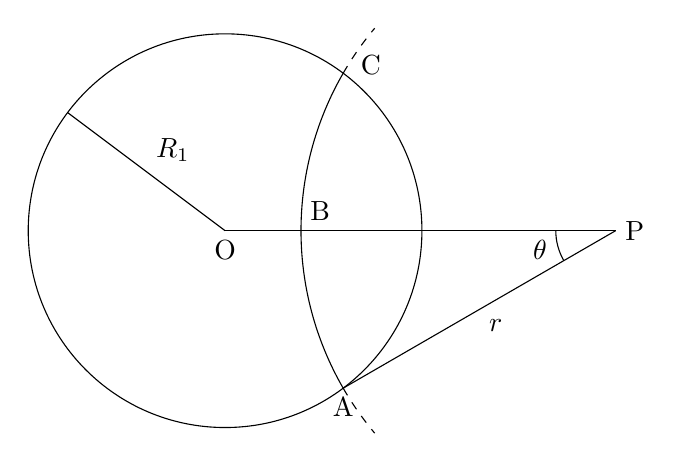
\begin{tikzpicture}
	\draw (0,0) circle (2.5);
	\draw (0,0) -- node[midway,anchor=south west] {$R_1$} (-2,1.5);
	\draw (0,0) node[anchor=north] {O} -- (4.96,0) node[anchor=west] {P};
	\draw (4.96,0) -- node[midway,anchor=north west] {$r$} (1.5,-2) node[anchor=north] {A};
	\draw (1.5,-2) arc (210:150:4);
	\draw[dashed] (1.5,-2) arc (210:220:4);
	\draw[dashed] (1.5,2) arc (150:140:4);
	\node[anchor=south west] at (0.96,0) {B};
	\node[anchor=west] at (1.6,2.1) {C};
	\node[anchor=north] at (4,0) {$\theta$};
	\draw (4.2,0) arc (180:210:0.76);
	\end{tikzpicture}
	\caption{}
	\label{fig:对一个球积分}
\end{figure}

现在考虑两个球之间的相互作用势能. 只需要对另一个球进行类似的操作
(所取的体积元中每个分子对第一个球的相互作用势能都相同), 可以获得
\begin{equation}
	\label{eq:待积分}
	E=\int_{z-R_2}^{z+R_2}E_\mathrm P\!\left(R\right)\cdot q_2\cdot
	\pi\frac Rz\left(R_1^2-\left(z-R\right)^2\right)\mathrm dR.
\end{equation}
将式 \ref{eq:球对分子的势能} 代入 \ref{eq:待积分} 后可积分得 (这一步不积出来也可以获得满分)
\begin{equation}
	E=-\frac{\pi^2q_1q_2\lambda}6\left(\frac{2R_1R_2}{z^2-\left(R_1+R_2\right)^2}
	+\frac{2R_1R_2}{z^2-\left(R_1-R_2\right)^2}
	+\ln\frac{z^2-\left(R_1+R_2\right)^2}{z^2-\left(R_1-R_2\right)^2}\right).
\end{equation}

将相互作用势能对 $z$ 求导后可获得相互作用力
\begin{equation}
	\label{eq:相互作用力}
	F=-\frac{\mathrm dE}{\mathrm dz}=
	-\frac{32\pi^2q_1q_2\lambda R_1^3R_2^3z}
	{3\left(z^2-\left(R_1+R_2\right)^2\right)^2\left(z^2-\left(R_1-R_2\right)^2\right)^2}.
\end{equation}
其相反数即为吸引力的大小.

\mypara
先考虑无限厚的墙.
将墙看作半径很大的球.
在式 \ref{eq:相互作用力} 中取
\begin{equation}
	z=d+R+R_2,\qquad R_1=R,\qquad R_2\to+\infty,\qquad q_1=q_2=q,
\end{equation}
可得
\begin{equation}
	-\frac{32\pi^2q^2\lambda R^3}3\lim_{R_2\to+\infty}
	\frac{R_2^3\left(d+R+R_2\right)}
	{\left(\left(d+R+R_2\right)^2-\left(R_2+R\right)^2\right)^2
	\left(\left(d+R+R_2\right)^2-\left(R_2-R\right)^2\right)^2}
	=-\frac{2\pi^2q^2\lambda R^3}{3d^2\left(d+2R\right)^2}.
\end{equation}

然后, 从无限厚的墙中挖掉一块无限厚的墙, 就可以得到一块有限厚的墙.
得到相互作用力
\begin{equation}
	F=-\frac{2\pi^2q^2\lambda R^3}{3}\left(\frac1{d^2\left(d+2R\right)^2}
	-\frac1{\left(d+t\right)^2\left(d+t+2R\right)^2}\right).
\end{equation}
其相反数即为吸引力的大小.
(若考生未写出答案, 但表达出了用无限大的球来表示无限厚的墙, 挖掉一块表示有限厚的墙,
则也可获得满分.)

\subsection{Moiré 纹}

\mypara
首先应当注意到 $d<p$ 与 $d>p$ 两种情况能给出定性上不同的条纹,
如图 \ref{fig:moire1} 所示.
可以看出, 当 $d>p$ 时会产生 $I=0$ 的区域, 而 $d<p$ 时则不会.

\begin{figure}[h!]
	\centering
	\begin{subfigure}{\linewidth}
		\centering
		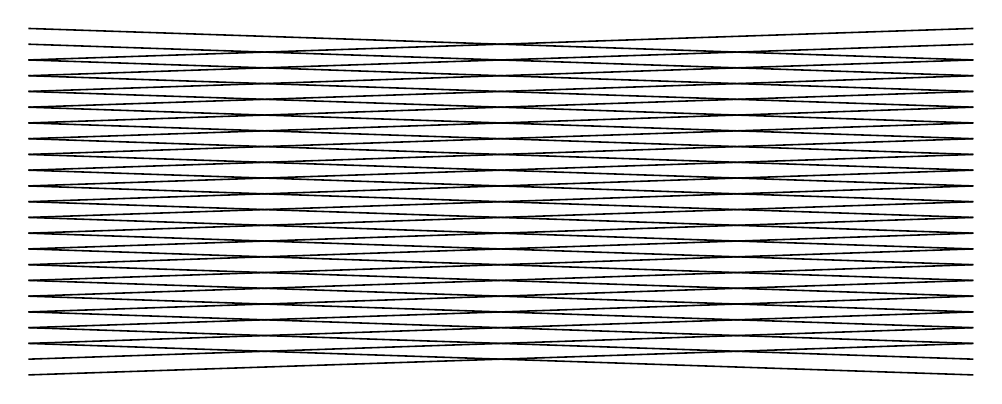
\begin{tikzpicture}
		\foreach \y in {0,...,20} {
			\draw[line width=0.02cm] (-6,0.2*\y) -- (6,0.2*\y+0.4);
			\draw[line width=0.02cm] (-6,0.2*\y+0.4) -- (6,0.2*\y);
		}
		\end{tikzpicture}
		\caption{$d<p$.}
		\label{fig:moire1a}
	\end{subfigure}
	\begin{subfigure}{\linewidth}
		\centering
		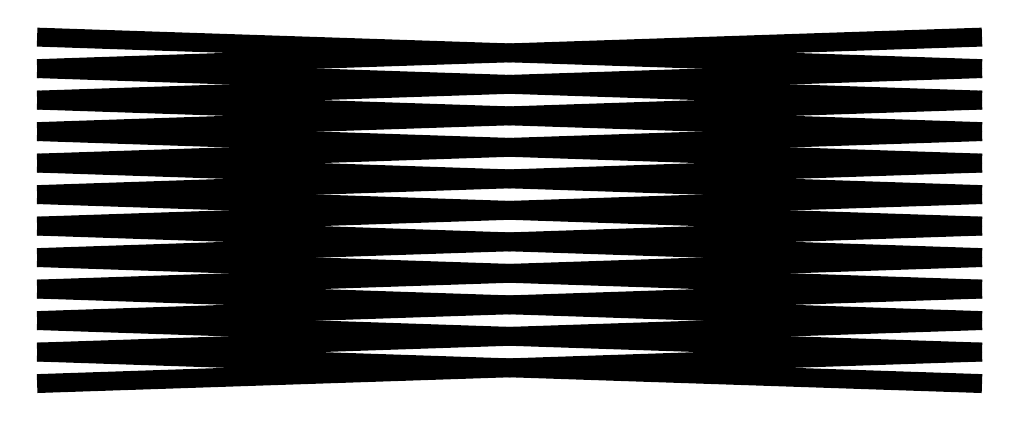
\begin{tikzpicture}
		\foreach \y in {0,...,10} {
			\draw[line width=0.24cm] (-6,0.4*\y) -- (6,0.4*\y+0.4);
			\draw[line width=0.24cm] (-6,0.4*\y+0.4) -- (6,0.4*\y);
		}
		\end{tikzpicture}
		\caption{$d>p$.}
		\label{fig:moire1b}
	\end{subfigure}
	\caption{}
	\label{fig:moire1}
\end{figure}

现在先研究 $d<p$ 的情形.
其平面几何如图 \ref{fig:moire1ageo} 所示.
阴影部分表示能遮挡光的部分.

\begin{figure}[h!]
	\centering
	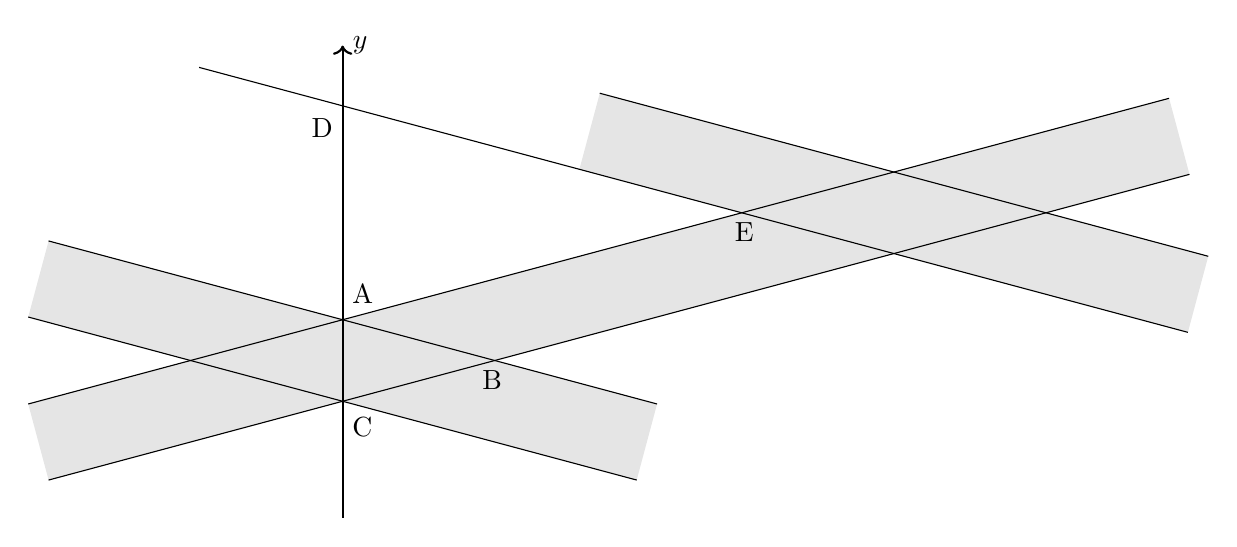
\begin{tikzpicture}
	\fill[rotate around={15:(0,0)},gray!20] (-4,0.5) rectangle (11,-0.5);
	\fill[rotate around={-15:(7,1.876)},gray!20] (3,2.376) rectangle (11,1.376);
	\fill[rotate around={-15:(0,0)},gray!20] (-4,0.5) rectangle (4,-0.5);
	\draw[rotate around={15:(0,0)}] (-4,0.5) -- (11,0.5);
	\draw[rotate around={15:(0,0)}] (-4,-0.5) -- (11,-0.5);
	\draw[rotate around={-15:(7,1.876)}] (3,2.376) -- (11,2.376);
	\draw[rotate around={-15:(7,1.876)}] (-2,1.376) -- (11,1.376);
	\draw[rotate around={-15:(0,0)}] (-4,0.5) -- (4,0.5);
	\draw[rotate around={-15:(0,0)}] (-4,-0.5) -- (4,-0.5);
	\draw[thick,->] (0,-2) -- (0,4) node[anchor=west] {$y$};
	\node[anchor=south west] at (0,0.6) {A};
	\node[anchor=north] at (1.9,0) {B};
	\node[anchor=north west] at (0,-0.6) {C};
	\node[anchor=north east] at (0,3.2) {D};
	\node[anchor=north] at (5.1,1.876) {E};
	\end{tikzpicture}
	\caption{}
	\label{fig:moire1ageo}
\end{figure}

显然, 三角形 ABC 是以 AC 为底边的等腰三角形, 其顶角 $\angle\mathrm{ABC}=2\theta$,
其腰上的高为 $d$.
经过一些初等的平面几何推导可知, 其底边上的高
\begin{equation}
	x_\mathrm B=\frac d{2\sin\theta}.
\end{equation}
在三角形 ADE 中经过类似的推导可知
\begin{equation}
	x_\mathrm E=\frac p{2\sin\theta}.
\end{equation}

取四边平行于坐标轴的矩形作为 $\mathrm dS$,
注意到矩形的高必然远大于 $d+p$,
同时矩形的宽必然远小于 $x_\mathrm B$.
显然当 $x=0$ 时, 亮度
\begin{equation}
	I=\frac{\left|\mathrm{AD}\right|}{\left|\mathrm{CD}\right|}
	=\frac p{p+d}.
\end{equation}
而当 $x\in\left[x_\mathrm B,x_\mathrm E\right]$ 时, 亮度
\begin{equation}
	I=1-\frac{2d}{p+d}=\frac{p-d}{p+d}.
\end{equation}
当 $x\in\left[0,x_\mathrm B\right]$ 时, 亮度随 $x$ 线性变化.

考虑到对称性, 可以知道 $I$ 是只与 $x$ 有关的以 $x_\mathrm B+x_\mathrm E$ 为周期的周期函数.
可以作出 $I$ 在一个周期上的函数图像, 如图 \ref{fig:moire1agraph} 所示.

\begin{figure}[h!]
	\centering
	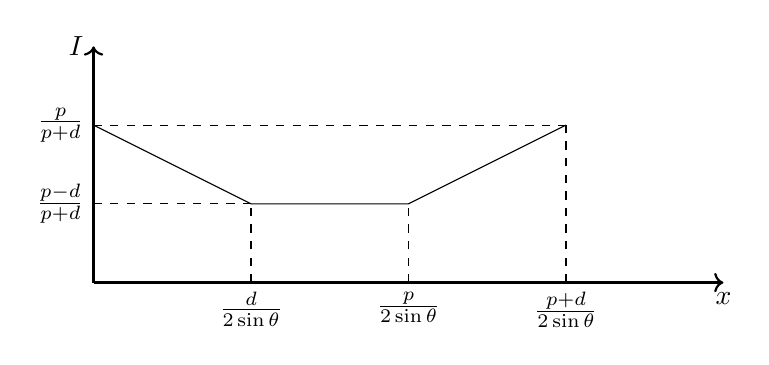
\begin{tikzpicture}
	\draw[thick,->] (0,0) -- (8,0) node[anchor=north] {$x$};
	\draw[thick,->] (0,0) -- (0,3) node[anchor=east] {$I$};
	\draw (0,2) -- (2,1) -- (4,1) -- (6,2);
	\draw[dashed] (0,1) node[anchor=east] {$\frac{p-d}{p+d}$} -- (2,1);
	\draw[dashed] (2,0) node[anchor=north] {$\frac d{2\sin\theta}$} -- (2,1);
	\draw[dashed] (4,0) node[anchor=north] {$\frac p{2\sin\theta}$} -- (4,1);
	\draw[dashed] (6,0) node[anchor=north] {$\frac{p+d}{2\sin\theta}$} -- (6,2);
	\draw[dashed] (0,2) node[anchor=east] {$\frac p{p+d}$} -- (6,2);
	\end{tikzpicture}
	\caption{}
	\label{fig:moire1agraph}
\end{figure}

观察图像可知, 可以利用绝对值函数将 $I$ 在一个周期上的解析式写出.
即, 当 $x\in\left[0,\frac{p+d}{2\sin\theta}\right)$ 时,
\begin{equation}
	\label{eq:moire1aI周期}
	I=\frac{\left|2x\sin\theta-d\right|+\left|2x\sin\theta-p\right|+p-d}
	{2\left(p+d\right)}.
\end{equation}

现在考虑 $d>p$ 的情形.
它与 $d<p$ 的区别在于, 在 $x$ 达到 $\frac d{2\sin\theta}$ 之前,
$x$ 会先达到 $\frac p{2\sin\theta}$ 从而使得 $I=0$.
可以画出此时 $I$ 在一个周期上的函数图像, 如图 \ref{fig:moire1bgraph} 所示.

\begin{figure}[h!]
	\centering
	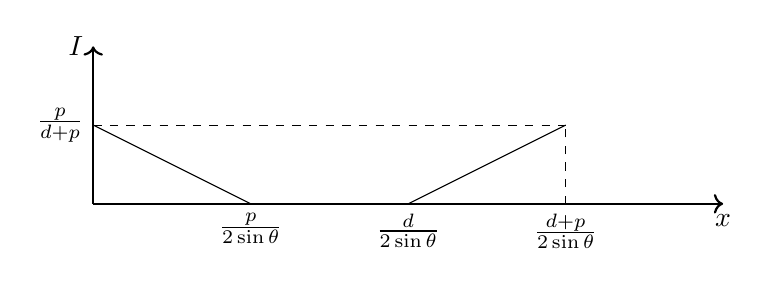
\begin{tikzpicture}
	\draw[thick,->] (0,1) -- (8,1) node[anchor=north] {$x$};
	\draw[thick,->] (0,1) -- (0,3) node[anchor=east] {$I$};
	\draw (0,2) -- (2,1) -- (4,1) -- (6,2);
	\draw[dashed] (2,1) node[anchor=north] {$\frac p{2\sin\theta}$} -- (2,1);
	\draw[dashed] (4,1) node[anchor=north] {$\frac d{2\sin\theta}$} -- (4,1);
	\draw[dashed] (6,1) node[anchor=north] {$\frac{d+p}{2\sin\theta}$} -- (6,2);
	\draw[dashed] (0,2) node[anchor=east] {$\frac p{d+p}$} -- (6,2);
	\end{tikzpicture}
	\caption{}
	\label{fig:moire1bgraph}
\end{figure}

观察图像可知, 可以利用绝对值函数将 $I$ 在一个周期上的解析式写出.
即, 当 $x\in\left[0,\frac{d+p}{2\sin\theta}\right)$ 时,
\begin{equation}
	\label{eq:moire1bI周期}
	I=\frac{\left|2x\sin\theta-p\right|+\left|2x\sin\theta-d\right|-\left(d-p\right)}
	{2\left(d+p\right)}.
\end{equation}
可以看出, 式 \ref{eq:moire1aI周期} 与式 \ref{eq:moire1bI周期} 其实是相同的.
因此它们同时适用于 $d<p$ 和 $d>p$ 的情况.

利用向下取整函数表达周期性.
于是 $\left(x,y\right)$ 处的亮度最终可以写为
\begin{equation}
	I\!\left(x,y\right)=\frac12\left(\left|
		\frac{2x\sin\theta-d}{p+d}-\left\lfloor\frac{2x\sin\theta}{p+d}\right\rfloor
	\right|+\left|
		\frac{2x\sin\theta-p}{p+d}-\left\lfloor\frac{2x\sin\theta}{p+d}\right\rfloor
	\right|+\frac{p-d}{p+d}\right).
\end{equation}

\mypara
若沿用上一问的做法, 利用平面几何来进行分析的话, 会过于困难.
这一问中, 由于条纹的间距和宽度相同, 因此可以从相位的角度考虑.

将 $\left(a,0\right)$ 与 $\left(-a,0\right)$ 假想为两个光源,
它们分别发出波长为 $d_+$ 和 $d_-$ 的光.
当光相遇的时候, 如果它们的相位差为 $2\pi$ 的整数倍, 则这里是亮纹中心 ($I=1/2$);
如果它们的相位差为 $\pi$ 的奇数倍, 则这里是暗纹中心 ($I=0$).
这是因为, 当相位差为 $2\pi$ 的整数倍的时候, 条纹刚好重合, 从而未被遮挡的区域刚好占了剩下的一半面积.
当相位差为 $\pi$ 的奇数倍的时候, 条纹刚好交错, 从而所有的区域都被遮挡.
这在图 \ref{fig:moire2} 中可以看出.
于是, 该问题被等效为一个波动光学问题.

\begin{figure}[h!]
	\centering
	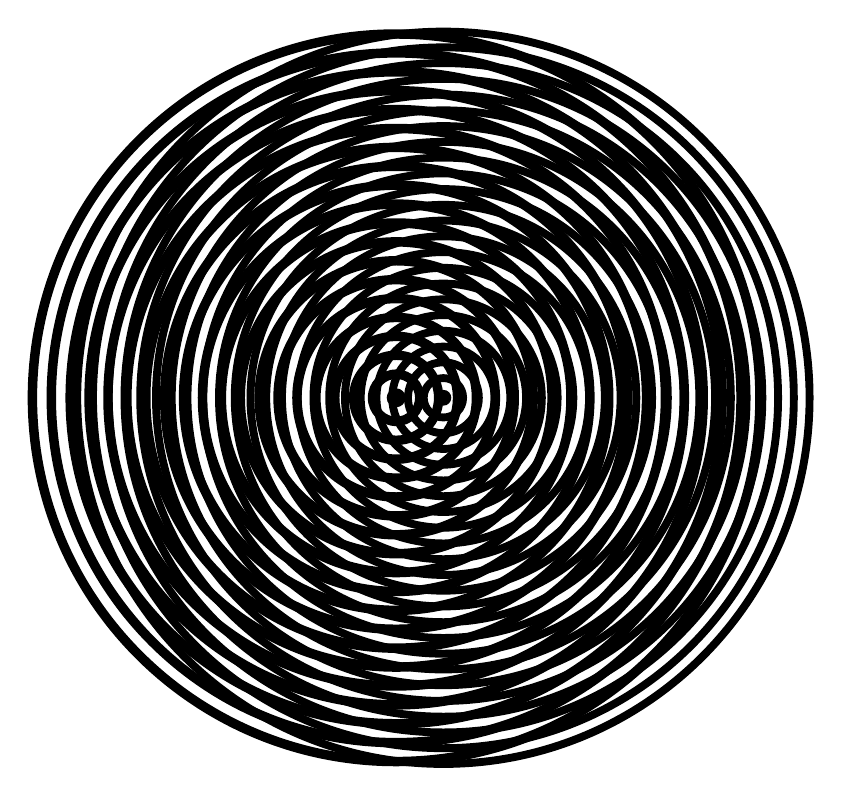
\begin{tikzpicture}
	\foreach \r in {0,...,23} {
		\fill[black,even odd rule] (0.3,0) circle (2*\r*0.1) (0.3,0) circle (2*\r*0.1+0.1);
	}
	\foreach \r in {0,...,19} {
		\fill[black,even odd rule] (-0.3,0) circle (2*\r*0.12) (-0.3,0) circle (2*\r*0.12+0.12);
	}
	\end{tikzpicture}
	\caption{}
	\label{fig:moire2}
\end{figure}

又, 注意到亮度应当随相位线性变化 (除非跨越 $\pi$ 的整数倍).
因此, 亮度关于相位差的函数是一个三角波
\begin{equation}
	\label{eq:亮度关于相位差}
	I=\frac14+\frac1{2\pi}\arcsin\cos\varphi.
\end{equation}
而相位差可以表示为
\begin{equation}
	\label{eq:相位差关于坐标}
	\frac\varphi\pi=\frac{\sqrt{\left(x+a\right)^2+y^2}}{d_-}-
	\frac{\sqrt{\left(x-a\right)^2+y^2}}{d_+}
	=\frac{d_+-d_-}{d_+d_-}\sqrt{x^2+y^2}
	+\frac{\left(d_++d_-\right)ax}{d_+d_-\sqrt{x^2+y^2}}.
\end{equation}
将式 \ref{eq:相位差关于坐标} 代入式 \ref{eq:亮度关于相位差} 可得
\begin{equation}
	I\!\left(x,y\right)=\frac14+\frac1{2\pi}\arcsin\cos\!\left(
	\frac{d_+-d_-}{d_+d_-}\pi\sqrt{x^2+y^2}
	+\frac{\left(d_++d_-\right)\pi ax}{d_+d_-\sqrt{x^2+y^2}}\right).
\end{equation}

\mypara
暗纹即
\begin{equation}
	\label{eq:暗纹}
	\varphi=\left(2n+1\right)\pi,\quad n\in\mathbb Z.
\end{equation}
将式 \ref{eq:相位差关于坐标} 代入式 \ref{eq:暗纹} 即可获得直角坐标下的暗纹方程
\begin{equation}
	\frac{d_+-d_-}{d_+d_-}\sqrt{x^2+y^2}
	+\frac{\left(d_++d_-\right)ax}{d_+d_-\sqrt{x^2+y^2}}=2n+1,
	\quad n\in\mathbb Z.
\end{equation}
从而可以获得极坐标下的方程
\begin{equation}
	\label{eq:极坐标暗纹方程}
	\frac{d_+-d_-}{d_+d_-}r
	+\frac{d_++d_-}{d_+d_-}a\cos\theta=2n+1,
	\quad n\in\mathbb Z.
\end{equation}

注意到式 \ref{eq:极坐标暗纹方程} 左边最小只能取 $-\frac{d_++d_-}{d_+d_-}a$,
因此 $n$ 有下界
\begin{equation}
	n_{\mathrm{min}}=\left\lceil-\frac{d_++d_-}{2d_+d_-}a-\frac12\right\rceil.
\end{equation}
大多数情况下式 \ref{eq:极坐标暗纹方程} 左边是没有最大值的, 从而 $n$ 可以取得任意大.
但是在
\begin{equation}
	d_+=d_-=:d
\end{equation}
时, 式 \ref{eq:极坐标暗纹方程} 左边有最大值 $2a/d$, 从而 $n$ 有上界
\begin{equation}
	n_{\mathrm{max}}=\left\lfloor\frac ad-\frac12\right\rfloor,
\end{equation}
于是只能有有限个 $n$, 从而暗纹的数量有限.
暗纹的数量
\begin{equation}
	m=n_{\mathrm{max}}-n_{\mathrm{min}}+1
	=2\left\lfloor\frac ad+\frac12\right\rfloor.
\end{equation}

\subsection{磁感线的秘密}

沿着曲线 $C_{k,n}$ 取线微元, 可以获得 $\left(x,y,z\right)$ 处的磁感应强度的方向
\begin{equation}
	\begin{cases}4x\,\mathrm dx+2y\,\mathrm dy=0,\\\mathrm dz=0\end{cases}
	\Rightarrow\mathbf B\!\left(x,y,z\right)\parallel
	\left[\begin{matrix}-y\\2x\\0\end{matrix}\right],
\end{equation}
从而可以设出
\begin{equation}
	\mathbf B\!\left(x,y,z\right)=
	u\!\left(x,y,z\right)\left[\begin{matrix}-y\\2x\\0\end{matrix}\right].
\end{equation}
由磁场的 Gauss 定理 $\nabla\cdot\mathbf B=0$ 可以得出关于 $u$ 的偏微分方程
\begin{equation}
	-y\frac{\partial u}{\partial x}+2x\frac{\partial u}{\partial y}=0.
\end{equation}
使用特征方程法或者分离变量法, 可以解出该方程的通解
\begin{equation}
	u=\Phi\!\left(2x^2+y^2\right),
\end{equation}
其中 $\Phi$ 是一个任意的可导函数.

现在确定 $\Phi$ 的形式.
为此, 考虑 $x=0$ 平面上穿过的磁感线.
$\mathbf B\!\left(0,y,z\right)$ 的大小应当正比于
$\left(0,y,z\right)$ 处穿过 $x=0$ 平面上单位面积的磁感线条数
(用 $\mathrm dk\,\mathrm dn$ 描述),
因为该处的磁场显然是垂直于 $x=0$ 平面的.
对于 $x=0$, 我们有
\begin{equation}
	\begin{cases}y=k^2R,\\z=nR\end{cases}\Rightarrow
	\begin{cases}\mathrm dy=2kR\,\mathrm dk,\\\mathrm dz=R\,\mathrm dn,\end{cases}
\end{equation}
从而
\begin{equation}
	-y\Phi\!\left(y^2\right)=B\propto\frac{\mathrm dk\,\mathrm dn}{\mathrm dy\,\mathrm dz}
	=\frac1{2R^2k}\propto y^{-\frac12},
\end{equation}
于是可以获得
\begin{equation}
	\Phi\!\left(y^2\right)\propto y^{-\frac32}=\left(y^2\right)^{-\frac34}.
\end{equation}
从而获得了 $\Phi$ 的形式.

将 $\Phi$ 的形式代入即可获得 $\mathbf B$ 的形式
\begin{equation}
	\mathbf B\propto\left(2x^2+y^2\right)^{-\frac34}
	\left[\begin{matrix}-y\\2x\\0\end{matrix}\right].
\end{equation}
由 Ampère 环路定理 $\nabla\times\mathbf B=\mu_0\mathbf j$ 可知,
通过对 $\mathbf B$ 求旋度, 可以获得 $\mathbf j$ 的形式.
显然它只有 $z$ 方向的分量
\begin{equation}
	j_z\propto\frac{\partial B_y}{\partial x}-\frac{\partial B_x}{\partial y}
	\propto y^2\left(2x^2+y^2\right)^{-\frac74}.
\end{equation}
再考虑到已知条件 $\left(0,R,0\right)$ 处 $j_z=j_0$, 可以获得答案
\begin{equation}
	\mathbf j\!\left(x,y,z\right)=\left[\begin{matrix}0\\0\\
	j_0R^{\frac32}y^2\left(2x^2+y^2\right)^{-\frac74}\end{matrix}\right].
\end{equation}

\subsection{老火箭题了}

此解答采用自然单位制 $c=1$.

设飞船的固有时为 $t'$.
显然有
\begin{equation}
	\label{eq:地面时固有时关系}
	\mathrm dt'=\sqrt{1-\dot x^2}\,\mathrm dt.
\end{equation}

飞船在固有时 $t'$ 时刻发射出质量为 $\mu\,\mathrm dt'$ 的推进剂, 考虑为质点分裂问题:
质量为 $M$ 的飞船分裂为质量为 $\mu\,\mathrm dt'$ 的推进剂和质量为 $M+\mathrm dM$ 的飞船.
固有时 $t'$ 时刻的瞬时静止系即为零动量系.
设飞船喷出推进剂后瞬间的速度为 $\mathrm dv'$.
于是有能量守恒
\begin{equation}
	\label{eq:能量守恒}
	M=M+\mathrm dM+\frac{\mu\,\mathrm dt'}{\sqrt{1-u^2}}
\end{equation}
和动量守恒 (已略去高阶小)
\begin{equation}
	\label{eq:动量守恒}
	0=M\,\mathrm dv'+\frac{\mu\,\mathrm dt'\cdot\left(-u\right)}{\sqrt{1-u^2}}.
\end{equation}
由式 \ref{eq:能量守恒} 可知 $\mathrm dM/\mathrm dt'=-\mu/\sqrt{1-u^2}$ 为一常量,
因此有
\begin{equation}
	\label{eq:质量固有时关系}
	M=m-\frac{\mu t'}{\sqrt{1-u^2}},
\end{equation}
其中 $m$ 是已知的初始质量.
将式 \ref{eq:质量固有时关系} 代入式 \ref{eq:动量守恒} 后可以获得
\begin{equation}
	\label{eq:v'}
	\mathrm dv'=\frac{u\mu\,\mathrm dt'}{m\sqrt{1-u^2}-\mu t'}.
\end{equation}

利用相对论速度变换公式可得地面系中分裂后瞬间的速度
\begin{equation}
	\label{eq:地面速度}
	\dot x+\mathrm d\dot x=\frac{\dot x+\mathrm dv'}{1+\dot x\,\mathrm dv'}
	=\dot x+\left(1-\dot x^2\right)\mathrm dv'.
\end{equation}
将式 \ref{eq:v'} 代入式 \ref{eq:地面速度} 可得
\begin{equation}
	\label{eq:dv/dt'}
	\mathrm d\dot x=\left(1-\dot x^2\right)\frac{u\mu\,\mathrm dt'}{m\sqrt{1-u^2}-\mu t'}.
\end{equation}
将式 \ref{eq:dv/dt'} 两边除以 $\mathrm dt$, 注意到式 \ref{eq:地面时固有时关系}, 可得
\begin{equation}
	\label{eq:加速度}
	\ddot x=\left(1-\dot x^2\right)^{\frac32}\frac{u\mu}{m\sqrt{1-u^2}-\mu t'},
\end{equation}
变形得
\begin{equation}
	m\sqrt{1-u^2}-\mu t'=u\mu\frac{\left(1-\dot x^2\right)^{\frac32}}{\ddot x}.
\end{equation}
两边对 $t$ 求导, 运用式 \ref{eq:地面时固有时关系}, 得
\begin{equation}
	-\mu\sqrt{1-\dot x^2}=u\mu
	\frac{-3\sqrt{1-\dot x^2}\dot x\ddot x^2-\left(1-\dot x^2\right)^{\frac32}\dddot x}{\ddot x^2},
\end{equation}
整理得
\begin{equation}
	\label{eq:x微分方程}
	\ddot x^2=u\left(3\dot x\ddot x^2-\left(1-\dot x^2\right)\dddot x\right).
\end{equation}
令 $v:=\dot x$, $a:=\ddot x$, 则有 $\dddot x=a\,\mathrm da/\mathrm dv$.
从而式 \ref{eq:x微分方程} 变为
\begin{equation}
	a^2=u\left(3a^2v+\left(1-v^2\right)a\frac{\mathrm da}{\mathrm dv}\right),
\end{equation}
分离变量得
\begin{equation}
	\frac{u\,\mathrm da}{a}=\frac{1-3uv}{1-v^2}\,\mathrm dv,
\end{equation}
积分得
\begin{equation}
	\label{eq:首次积分}
	u\ln\frac a{a_0}=\frac{3u+1}2\ln\!\left(1+v\right)+\frac{3u-1}2\ln\!\left(1-v\right),
\end{equation}
其中 $a_0$ 为初始的加速度, 可以通过在式 \ref{eq:加速度} 中代入 $\dot x=0$, $t'=0$ 获得
\begin{equation}
	\label{eq:a0}
	a_0:=\left.\ddot x\right|_{\dot x=0,~t'=0}=\frac\mu m\frac u{\sqrt{1-u^2}}.
\end{equation}
将式 \ref{eq:a0} 代入式 \ref{eq:首次积分} 并整理可得
\begin{equation}
	\frac{\mathrm dv}{\mathrm dt}=a=\frac\mu m\frac u{\sqrt{1-u^2}}
	\left(1+v\right)^{\frac1{2u}+\frac32}\left(1-v\right)^{-\frac1{2u}+\frac32}.
\end{equation}
分离变量并积分, 得
\begin{equation}
	\label{eq:使用积分公式前}
	t=\frac m\mu\frac{\sqrt{1-u^2}}u\int_0^v\left(1+\xi\right)^{-\frac1{2u}-\frac32}
	\left(1-\xi\right)^{\frac1{2u}-\frac32}\,\mathrm d\xi.
\end{equation}
注意到 $-\frac1{2u}\ne\pm\frac12$, 可以运用题目所给的积分公式得出
\begin{equation}
	t=\frac m\mu\frac{1-\left(1+uv\right)\left(1+v\right)^{-\frac1{2u}-\frac12}
	\left(1-v\right)^{\frac1{2u}-\frac12}}{\sqrt{1-u^2}}.
\end{equation}

\textit{另}: 可以直接在地面系中考虑质点分裂的过程.

设原本质量为 $M$ 的飞船分裂为质量为 $M+\mathrm dM$ 的飞船和质量为 $\mu\,\mathrm dt'$ 的推进剂.
分裂前飞船的速度为 $v$, 分裂后飞船的速度为 $v+\mathrm dv$.
分裂后推进剂在速度为 $v$ 的参考系中的速度为 $-u$, 因此它在地面系中的速度为
$\left(v-u\right)/\left(1-uv\right)$.
由此列出能量守恒
\begin{equation}
	\label{eq:能量守恒2}
	\mathrm d\!\left(\frac M{\sqrt{1-v^2}}\right)+
	\frac{\mu\,\mathrm dt'}{\sqrt{1-\left(\frac{v-u}{1-uv}\right)^2}}=0
\end{equation}
和动量守恒
\begin{equation}
	\label{eq:动量守恒2}
	\mathrm d\!\left(\frac{Mv}{\sqrt{1-v^2}}\right)+
	\frac{\mu\,\mathrm dt'\frac{v-u}{1-uv}}{\sqrt{1-\left(\frac{v-u}{1-uv}\right)^2}}=0.
\end{equation}

由式 \ref{eq:能量守恒2} 和式 \ref{eq:动量守恒2} 联立可得
\begin{equation}
	\label{eq:E,v微分方程}
	\mathrm d\!\left(Ev\right)=\frac{v-u}{1-uv}\,\mathrm dE,
\end{equation}
其中
\begin{equation}
	\label{eq:飞船E}
	E:=\frac M{\sqrt{1-v^2}}.
\end{equation}
将式 \ref{eq:E,v微分方程} 分离变量可得
\begin{equation}
	\frac{\mathrm dE}E=\frac{\mathrm dv}{\frac{v-u}{1-uv}-v},
\end{equation}
积分得
\begin{equation}
	\label{eq:首次积分2}
	\ln\frac E{E_0}=\frac{-1-u}{2u}\ln\!\left(1+v\right)
	+\frac{1-u}{2u}\ln\!\left(1-v\right),
\end{equation}
其中 $E_0$ 为 $E$ 的初始值, 可以通过在式 \ref{eq:飞船E} 中代入 $M=m$, $v=0$ 获得
\begin{equation}
	\label{eq:E0}
	E_0:=\left.E\right|_{M=m,~v=0}=m.
\end{equation}
将式 \ref{eq:E0} 代入式 \ref{eq:首次积分2} 后可整理得
\begin{equation}
	\label{eq:E关于v}
	E=m\left(1+v\right)^{-\frac1{2u}-\frac12}\left(1-v\right)^{\frac1{2u}-\frac12}.
\end{equation}

式 \ref{eq:能量守恒2} 给出
\begin{equation}
	\label{eq:dt'关于dE}
	\mu\,\mathrm dt'=-\sqrt{1-\left(\frac{v-u}{1-uv}\right)^2}\,\mathrm dE.
\end{equation}
将式 \ref{eq:地面时固有时关系} 与式 \ref{eq:E关于v} 代入式 \ref{eq:dt'关于dE} 后, 可整理得
\begin{equation}
	\mu\,\mathrm dt=\frac{\sqrt{1-u^2}}um\left(1+v\right)^{-\frac1{2u}-\frac32}
	\left(1-v\right)^{\frac1{2u}-\frac32}\,\mathrm dv,
\end{equation}
由此分离变量并积分可以得出与式 \ref{eq:使用积分公式前} 相同的式子.

\subsection{死亡半径}

首先写出势能.
势能即为粒子与像电荷之间的相互作用势能
\begin{equation}
	U\!\left(r\right)=\frac12q\frac{-\frac Rrq}
	{4\pi\varepsilon_0\left(r-\frac{R^2}r\right)}
	=-\frac12mv^2\frac{a^2}{r^2-R^2},
\end{equation}
其中常数
\begin{equation}
	a:=\sqrt{\frac{q^2R}{4\pi\varepsilon_0mv^2}}
\end{equation}
具有长度量纲.

设粒子的瞄准距离 (初速度所在直线与球心的距离) 为 $\rho$.
则粒子的能量和角动量分别为
\begin{equation}
	E=\frac12mv^2,\qquad L=m\rho v,
\end{equation}
于是可以写出径向运动的有效势能
\begin{equation}
	V\!\left(r\right)=U\!\left(r\right)+\frac{L^2}{2mr^2}
	=\frac12mv^2\left(-\frac{a^2}{r^2-R^2}+\frac{\rho^2}{r^2}\right).
\end{equation}
粒子的活动范围由 $V<E$ 给出
\begin{equation}
	\label{eq:活动范围不等式}
	-\frac{a^2}{r^2-R^2}+\frac{\rho^2}{r^2}<1.
\end{equation}
记式 \ref{eq:活动范围不等式} 的解集为 $r\in S$, 则粒子能撞到金属球的条件可被写为
$\left(R,+\infty\right)\subseteq S$.
实际上, 粒子的活动范围不仅不会超过 $S$, 还有可能不足 $S$,
这是因为 $S$ 可能不是连通的.
实际上粒子的活动范围只能是 $S$ 的最靠右 (数值最大) 的连通分量, 记作 $S^*$.

由于我们只需要考虑 $S$ 中 $r>R$ 的部分, 因此可以认为 $r^2-R^2>0$.
因此可以将式 \ref{eq:活动范围不等式} 两边同时乘 $\left(r^2-R^2\right)r^2$ 而保持不等号方向不变:
\begin{equation}
	-a^2r^2+\rho^2\left(r^2-R^2\right)<\left(r^2-R^2\right)r^2.
\end{equation}
这是一个关于 $r^2$ 的二次不等式, 其解集为
\begin{equation}
	r^2\in
	\begin{cases}\left(-\infty,r_-^2\right)\cup\left(r_+^2,+\infty\right),
	&\text{若 $\Delta\ge0$;}\\
	\mathbb R&\text{若 $\Delta<0$,}\end{cases}
\end{equation}
其中
\begin{equation}
	\label{eq:Delta,r_pm}
	\Delta:=\left(\frac{R^2-a^2+\rho^2}2\right)^2-\rho^2R^2,
	\qquad r_\pm^2:=\frac{R^2-a^2+\rho^2}2\pm\sqrt\Delta.
\end{equation}
因此, 如果想让 $\left(R,+\infty\right)\subseteq S$, 条件为
\begin{equation}
	\label{eq:条件1}
	\Delta\ge0\land r_+^2\le R^2
\end{equation}
或者
\begin{equation}
	\label{eq:条件2}
	\Delta<0.
\end{equation}

首先, 我们考虑式 \ref{eq:条件1}.
由 $\Delta\ge0$ 可解得
\begin{equation}
	\label{eq:条件1解集1}
	\rho^2\in\left(-\infty,\left(R-a\right)^2\right]
	\cup\left[\left(R+a\right)^2,+\infty\right).
\end{equation}
由 $r_+^2\le R^2$ 可解得
\begin{equation}
	\label{eq:条件1解集2}
	\rho^2\in\left(-\infty,R^2+a^2\right].
\end{equation}
将式 \ref{eq:条件1解集1} 与式 \ref{eq:条件1解集2} 取交集.
注意到 $R^2+a^2<\left(R+a\right)^2$, 于是可得
\begin{equation}
	\label{eq:条件1解集}
	\rho^2\in\left(-\infty,\left(R-a\right)^2\right].
\end{equation}
这就是式 \ref{eq:条件1} 的解集.

然后, 再考虑式 \ref{eq:条件2}.
容易解出它的解集为
\begin{equation}
	\label{eq:条件2解集}
	\rho^2\in\left(\left(R-a\right)^2,\left(R+a\right)^2\right).
\end{equation}

将式 \ref{eq:条件1解集} 与式 \ref{eq:条件2解集} 取并集, 可得粒子能撞击金属球的条件
\begin{equation}
	\rho^2<\left(R+a\right)^2.
\end{equation}
也就是说, 粒子不能撞击金属球的条件为
\begin{equation}
	\label{eq:不撞击条件}
	\rho^2\ge\left(R+a\right)^2.
\end{equation}
在式 \ref{eq:不撞击条件} 下, 我们可以获得粒子真正的活动范围
\begin{equation}
	\label{eq:真正的活动范围}
	S^*=\left(r_+,+\infty\right).
\end{equation}

现在考虑 $d$.
由题目所说, $d\in S^*$ 是粒子能撞击金属球的充分条件.
所以, $d\notin S^*$ 是粒子不能撞击金属球的必要条件.
也就是说, 用式 \ref{eq:不撞击条件} 的话来说, 就是
$\rho^2\ge\left(R+a\right)^2\Rightarrow d\notin S^*$.
也就是说,
\begin{equation}
	d\notin\bigcup_{\rho^2\ge\left(R+a\right)^2}S^*.
\end{equation}
因此, 题目所要求的 $d$ 的最大值即
\begin{equation}
	\label{eq:d_max}
	d_{\mathrm{max}}=\max\left(\mathbb R\setminus
	\bigcup_{\rho^2\ge\left(R+a\right)^2}S^*\right).
\end{equation}
因此, 若要获得 $d_{\mathrm{max}}$, 只需获得 $\bigcup_{\rho^2\ge\left(R+a\right)^2}S^*$.

根据式 \ref{eq:Delta,r_pm} 可以获得 $\Delta$ 对 $\rho^2$ 的导数
\begin{equation}
	\frac{\mathrm d\Delta}{\mathrm d\!\left(\rho^2\right)}=\frac{\rho^2-R^2-a^2}2.
\end{equation}
从而, 由式 \ref{eq:不撞击条件} 以及 $R^2+a^2<\left(R+a\right)^2$ 可知
$\mathrm d\Delta/\mathrm d\!\left(\rho^2\right)>0$.
从而, $\Delta$ 是关于 $\rho^2$ 的单调递增函数.
从而, 由式 \ref{eq:Delta,r_pm} 中 $r_+^2$ 的形式可以看出,
$r_+^2$ 也是关于 $\rho^2$ 的单调递增函数.
因此, $S^*$ 的范围随着 $\rho^2$ 的增大而缩小
(即, 更大的 $\rho^2$ 对应的 $S^*$ 是更小的 $\rho^2$ 对应的 $S^*$ 的子集).
因此, 所有 $S^*$ 的并集就是当 $\rho^2$ 最小时的 $S^*$.
因此, 将 $\rho^2=\left(R+a\right)^2$ 代入式 \ref{eq:Delta,r_pm},
再代入式 \ref{eq:真正的活动范围}, 即可获得
\begin{equation}
	\bigcup_{\rho^2\ge\left(R+a\right)^2}S^*=
	\left.S^*\right|_{\rho^2=\left(R+a\right)^2}=
	\left(\sqrt{R\left(R+a\right)},+\infty\right).
\end{equation}
将其代入式 \ref{eq:d_max} 后可获得
\begin{equation}
	\label{eq:d_max答案}
	d_{\mathrm{max}}=\sqrt{R\left(R+a\right)}=
	\sqrt{R\left(R+\sqrt{\frac{q^2R}{4\pi\varepsilon_0mv^2}}\right)}.
\end{equation}

\textit{另}: 此题有一个很物理的方法.

若粒子无法撞击到金属球, 则显然是因为径向运动的有效势能中存在势垒.
若粒子的能量不足以翻越势垒, 则无法撞击到金属球.

现在考虑临界情况: 粒子的能量刚好与势垒的高度相同.
此时粒子会在无限长的时间里无限接近势垒所在的位置而无法达到势垒.
这一过程使得粒子的运动无限接近于匀速圆周运动.
这个匀速圆周运动的轨迹的半径就是所要求的 $d_{\mathrm{max}}$,
因为一旦进入了半径为 $d_{\mathrm{max}}$ 的范围以内,
就可以断言粒子的能量高于势垒的高度而翻越了势垒.

现在, 假设一个初始时具有能量 $\frac12mv^2$ 的粒子在足够长的时间之后绕着金属球圆周运动,
圆周运动的角速度为 $\omega$, 半径为 $d_{\mathrm{max}}$.
由 Newton 第二定律得
\begin{equation}
	\frac{q\cdot\left(-\frac R{d_{\mathrm{max}}}q\right)}
	{4\pi\varepsilon_0\left(d_{\mathrm{max}}-\frac{R^2}{d_{\mathrm{max}}}\right)}
	=m\omega^2d_{\mathrm{max}}.
\end{equation}
由能量守恒得
\begin{equation}
	\frac12mv^2=\frac12md_{\mathrm{max}}^2\omega^2+\frac12q
	\frac{-\frac R{d_{\mathrm{max}}}q}
	{4\pi\varepsilon_0\left(d_{\mathrm{max}}-\frac{R^2}{d_{\mathrm{max}}}\right)}.
\end{equation}
联立成关于 $d_{\mathrm{max}}$ 和 $\omega$ 的方程组,
解得与式 \ref{eq:d_max答案} 相同的答案.

\end{document}
